\chapter{Decision Trees}
\label{cha:decision_trees}

\begin{figure}[H]
	\centering
	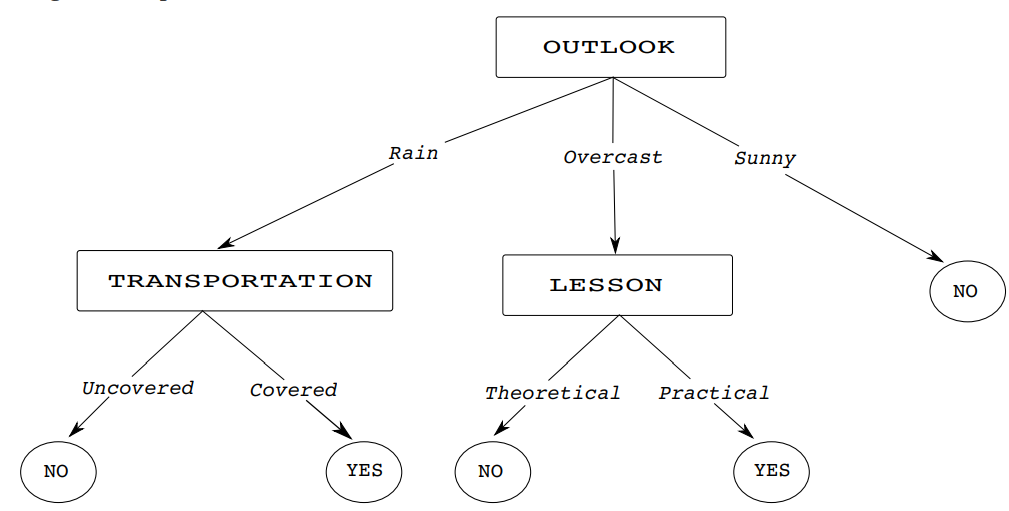
\includegraphics[width=0.8\textwidth]{
		images/02_DecisionTrees_decisionTree1.png
	}
	\caption{Toy example of a decision tree. \textit{Go to lesson}.}
	\label{dt_example}
\end{figure}

\defi{\textbf{Decision tree} \label{def:dt}\\ A \textit{decision tree} encodes a logical formula expressed in \textit{disjunctive normal form}. It consists of a disjunction of conjuctions of constraints over attribute values. Each path from the root to a leaf is a conjunction of the constraints specified in the nodes along it. The leaf contains the label to be assigned to instances reaching it. }
Given a decision three, such as the one reported in Figure \ref{dt_example}, the
disjunction of all paths is the logical formula represented by the tree.

% \begin{equation*}
% \begin{array}{l}
%     (\mathit{OUTLOOK}=\mathit{Rain} \wedge \mathit{TRANSPORTATION}=\mathit{Covered})\\
%     \vee \\
%     (\mathit{OUTLOOK}=\mathit{Overcast} \wedge \mathit{LESSON}=\mathit{Practical})
% \end{array}
% \end{equation*}

\begin{gather*}
	(\mathit{OUTLOOK}=\mathit{Rain}\wedge \mathit{TRANSPORTATION}=\mathit{Covered})
	\\ \vee \\ (\mathit{OUTLOOK}=\mathit{Overcast}\wedge \mathit{LESSON}=\mathit{Practical}
	)
\end{gather*}

\textbf{Remark:} the tree encodes a DNF formula for each class.
\newline

Appropriate problems for decision trees are:
\begin{itemize}
	\item Binary or multiclass classification tasks. Extensions to regressions
		also exists. The most simple regression extension is to predict the average of
		the training examples which reached a leaf.

	\item Instances represented as attribute-value pairs. Indeed the idea is to
		split according to attribute values.

	\item Different explanations for the concept are possible (disjunction). For
		example looking at decision tree in Figure \ref{dt_example}, there can be several
		reasons why I decide to attend a lecture. Decision trees allow to learn
		several explanations for a given concept.

	\item Some instances have missing attributes, i.e. for some attributes we do not
		have the value. This is typical in medical domain in which it is unlikely
		that a patient did all the possible tests which could be useful to make a
		prediction.

	\item There is need for an interpretable explanation of the output.
\end{itemize}

\begin{figure}[H]
	\centering
	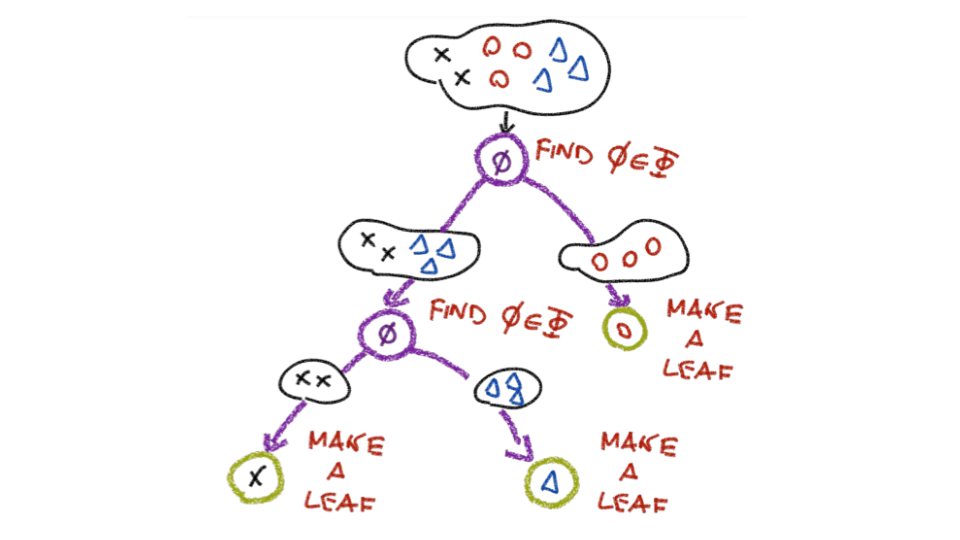
\includegraphics[width=0.7\textwidth]{
		images/02_DecisionTrees_decisionTree2.png
	}
	\caption{Split node training set into children according to the value of the
	chosen attribute}
	\label{ricci_dt}
\end{figure}

\section{Learning decision trees}
In order to learn a decision tree, we follow a \textit{greedy} top-down strategy
inspired by a \textit{divide et impera} approach. For each node, starting from the
root with full training set:
\begin{enumerate}
	\item Choose the best attribute to be evaluated

	\item Add a child for each attribute value

	\item Split node training set into children according to the value of the chosen
		attribute

	\item Stop splitting a node when a stopping condition is met. For example, the
		node which has been reached contains examples from a single class (all
		examples have the same label, they are homogeneous), or there are no more attributes
		to test.
\end{enumerate}

\textbf{Remark:} if the current set of examples is not homogeneous but we stop
splitting for other reasons, we assign to the leaf the majority class of the set.
\newline

In essence, the learning algorithm recursively partitions the training set and
decides whether to grow leaves or non-terminal nodes.

\subsection{Choosing the best attribute}

\defi{\textbf{Entropy} \label{def:entropy}\\ The \textit{entropy} is a measure of the amount of information contained in a collection of instances (training examples) $S$ which can take a number $c$ of possible values (class labels). The entropy of a set of labelled examples measures its label inhomogeneity. \begin{equation}H(S) = - \sum_{i=1}^{c}p_{i}\log_{2}{p_i}\end{equation} where $p_{i}$ is the fraction of $S$ taking value $i$. }

\defi{\textbf{Information gain} \label{def:information_gain}\\ \textit{Information gain} is the expected reduction of entropy obtained by partitioning a set $S$ according to the value of a certain attribute $A$. \begin{equation}\mathit{IG}(S,A) = H(S)-\sum_{v \in \mathit{Values}(A)}\frac{|S_{v}|}{|S|}H(S_{v})\end{equation} where $\mathit{Values}(A)$ is the set of possible values taken by $A$ and $S_{v}$ is the subset of $S$ taking value $v$ at attribute $A$. \begin{itemize}\item The second term represents the sum of entropies of subsets of examples obtained partitioning over $A$ values, weighted by their respective sizes.

\item An attribute with high information gain tends to produce homogeneous groups in terms of labels, thus favouring their classification.\end{itemize} \textbf{Remark:} \[IG(S,A) \geq 0\] }

Overall, the selection of the best splitting attribute is given in terms of
maximization of information gain. The procedure ends when the subset of the training
set which has reached a given node along the path from the root of the tree satisfies
a certain criterion. For instance, the set of training examples which has reached
the current node, is characterized by a homogeneity value lower then a given
threshold ($H(S)<\epsilon$), has a given minimum cardinality ($|S|<k$), is
completely homogeneous, there are no more splitting attributes to choose.
Depending on the particular implementation, in some of these cases we grow a leaf
instead of splitting the training examples and generating new intermediate nodes.

\section{Issues in decision tree learning}

\subsection{Overfitting avoidance}
Decision trees have a structure that is determined by the data. As a result they
are flexible and can easily fit the training set, with high risk of overfitting.\\
Requiring that each leaf has only examples of a certain class can lead to very
complex trees. A complex tree can easily overfit the training set, incorporating
random regularities not representative of the full distribution. What is more many
kinds of noise can occur in the training data: some values of attributes are
incorrect because of errors in the data acquisition process, the instance was labeled
incorrectly, some attributes are irrelevant to the decision making process. In order
to build simpler tree structures, less prone to overfitting, it is possible to accept
impure leaves, assigning them the label of the majority of their training
examples.\\ A technique to reduce complexity is called \textit{pruning}. There
are two possible strategies to prune a decision tree:
\begin{itemize}
	\item \textbf{pre-pruning}: decide whether to stop splitting a node even if it
		contains training examples with different labels.

	\item \textbf{post-pruning}: learn a full tree and successively prune it removing
		subtrees, replacing whole subtrees with leaf nodes.
\end{itemize}

With the aim of improving generalization and as a consequence, reducing overfitting,
if a \textit{validation set} is available it is possible to implement a post-pruning
strategy. The procedure is described in Algorithm \ref{alg:postPruning}.

\begin{algorithm}
	\caption{Post pruning \label{alg:postPruning}}
	\begin{algorithmic}
		[1] \STATE \textbf{for each} node $n$ in the tree \textbf{do}\{ \STATE \tab
		Evaluate the performance on the validation set \STATE \tab when removing the
		subtree rooted at $n$ \STATE \} \STATE \textbf{if} all node removals worsen performance\{
		\STATE \tab STOP \STATE \} \STATE \STATE $n$ $\leftarrow$ node whose removal
		has the best performance improvement \STATE \STATE Replace the subtree
		rooted at $n$ with a leaf \STATE \STATE Assign to the leaf the majority
		label of all examples in the subtree \STATE \STATE \textbf{return} to line 1
	\end{algorithmic}
\end{algorithm}

\subsection{Dealing with continuous-valued attributes}
Continuous valued attributes need to be discretized in order to be used in internal
nodes tests. Discretization threshold can be chosen to maximize the information
gain. A possible procedure is the following:
\begin{enumerate}
	\item Examples are sorted according to their continuous attribute values.

	\item For each pair of successive examples having different labels, a
		candidate threshold is placed as the average of the two attribute values.

	\item For each candidate threshold, the information gain achieved by splitting
		the examples is computed.

	\item The threshold producing the higher information gain is used to discretize
		the attribute.
\end{enumerate}

\subsection{Alternative attribute test measures}
The information gain criterion tends to prefer attributes with a large number of
possible values. As an extreme, the unique ID of each example is an attribute which
perfectly splits the data into singletons, but it will be of no use on new
examples. Moreover, this would lead to overfitting.
\paragraph{}
In order to deal with this problem a new measure of entropy is introduced. In this
case we do not compute entropy taking into account class values, but we
calculate the spread with respect to the values of the attributes.
\begin{equation}
	H_{A}(S) = -\sum_{v \in \mathit{Values}(A)}\frac{|S_{v}|}{|S|}\log_{2}{\frac{|S_{v}|}{|S|}}
\end{equation}
This quantity is maximized when there exists an attribute which splits the dataset
homogeneously in many subsets. The aim is to discourage the choice of these kind
of attributes to perform the splits. To do this \textit{gain ratio} is
introduced as an alternative of information gain measure introduced above.
\begin{equation}
	\mathit{IGR}(S,A) = \frac{\mathit{IG}(S,A)}{H_{A}(S)}
\end{equation}
In this case, splitting according to unique identifiers would result in high
values of entropy with respect to attribute values ($H_{A}(S)$), which leads to low
values of gain ratio ($\mathit{IGR}(S,A)$).

\subsection{Handling attributes with missing values}
Assume that an example $x$ with class $c(x)$ has missing value for attribute $A$.
When attribute $A$ has to be tested at node $n$, the following solutions could be
adopted:
\begin{itemize}
	\item \textit{Simple solution}. Assign to $x$ the most common attribute value among
		the examples in $n$ or (during training) the most common attribute value among
		the examples in $n$ with class $c(x)$.

	\item \textit{Complex solution}. Propagate $x$ to each of the children of $n$,
		with a fractional value equal to the proportion of examples with the
		corresponding attribute value.\\At training time, you assign the leaf the
		majority vote among the training examples which reach that leaf considering
		their weight.\\At test time, if we process an example with missing
		attributes it ends up in multiple leaves with a given probability. Each leaf
		votes with a weight which depends on the fraction of the test example which reached
		that leaf.
\end{itemize}

\begin{figure}[H]
	\centering
	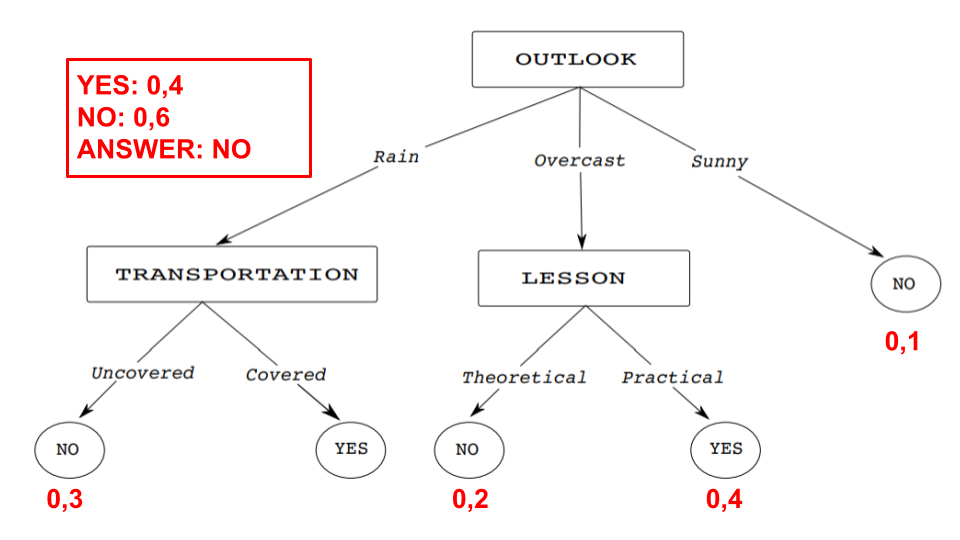
\includegraphics[width=0.8\textwidth]{
		images/02_DecisionTrees_missingAttributes.png
	}
	\caption{Dealing with missing attributes at test time. Complex solution.}
	\label{missing_attributes}
\end{figure}

\section{Random forest}

A common technique to reduce overfitting is \textit{ensemble learning}. Following
this method we learn multiple models at training time. At test time we average
the results or take the majority vote of the models.

\subsection{Bootstrap sampling and bagging}
\paragraph{}
\textbf{Bootstrap sampling:} Given a set $D$ containing $N$ training examples, create
$D'$ by drawing $N$ examples at random with replacement (i.e. same example can be
selected multiple times) from $D$.
\paragraph{}
\textbf{Bagging:}
\begin{enumerate}
	\item Create $k$ bootstrap datasets $D_{i}$

	\item Train distinct classifier on each $D_{i}$

	\item Classify new instance by majority vote/average
\end{enumerate}

\subsection{Training}
Random forests are ensembles of decision trees. Each tree is typically trained on
a bootstrapped version of the training set (sampled with replacement, i.e.
independent samples). Each decision tree is independently trained with its
bootstrapped version of the training set. At each node the splitting function is
optimized on $m$ randomly sampled features. This helps obtaining decorrelated
decision trees At the end of the training a forest with $M$ trees is generated.
\begin{figure}[H]
	\centering
	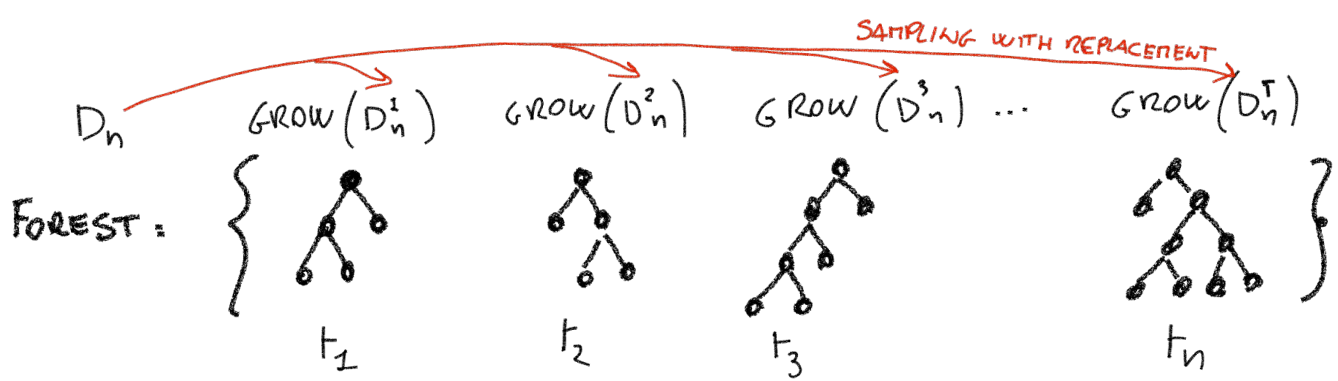
\includegraphics[width=\textwidth]{images/02_DecisionTrees_randomForest.png}
	\caption{Random forest}
	\label{rf}
\end{figure}

\subsection{Testing}
\begin{enumerate}
	\item Test the example with each tree in the forest.

	\item Return the majority class among the predictions.
\end{enumerate}
More formally, given a set of trees $Q=\{t_{1}, ..., t_{T}\}$, the final
prediction of the forst is obtained by averaging the prediction of each tree in
the ensemble:
\begin{equation}
	f_{Q}(x) = \frac{1}{T}\sum_{j=1}^{T}f_{t}(x)
\end{equation}
